\section{Results}
\subsection{The monetary bridge remains fiscally constrained}
Table~\ref{tab:bench} gives the medium-path year-50 comparisons. In B6, MVI is \ResultPSixMviGdp\% of GDP compared with \ResultPTwoMviGdp\% under B2. Conventional tax revenue nevertheless remains \ResultPSixTaxGdp\% of GDP. The hybrid is not a tax-free equilibrium. The baseline path has a small opening monetary contraction while balances and the levy adjust; negative issuance is retained in the data rather than relabelled as positive seigniorage.

\begin{table}[htbp]\centering\small
\caption{Medium automation at year 50; peak inflation covers the entire available path}\label{tab:bench}
\begin{tabular}{lllllll}
\toprule
Policy & Complete & Real GDP & MVI/GDP & Tax/GDP & Wealth Gini & Peak inflation \\
\midrule
B0 & yes & 6.48 & 7.1\% & 25.0\% & 0.768 & 2.1\% \\
B1 & yes & 6.48 & 0.0\% & 17.8\% & 0.788 & 2.0\% \\
B2 & yes & 6.48 & 19.0\% & 37.0\% & 0.754 & 2.2\% \\
B3 & yes & 6.48 & 12.4\% & 22.8\% & 0.800 & 40.3\% \\
B4 & yes & 6.48 & 12.0\% & 22.8\% & 0.804 & 45.1\% \\
B5 & yes & 6.48 & 10.6\% & 28.5\% & 0.583 & 2.1\% \\
B6 & yes & 6.48 & 10.2\% & 27.1\% & 0.584 & 2.1\% \\
B7 & yes & 6.48 & 6.0\% & 23.9\% & 0.560 & 2.1\% \\
B8 & yes & 6.46 & 11.0\% & 29.0\% & 0.578 & 8.6\% \\
B9 & no & -- & -- & -- & -- & -- \\
\bottomrule
\end{tabular}

\par\smallskip\footnotesize Real GDP is indexed to one initially. Missing year-50 values indicate a stopped numerical path. B9's extreme peak is a model-breakdown diagnostic, not a quantitative inflation forecast.
\end{table}

Fiscal dominance produces a materially different result. With the fixed 30\% factor-income tax, B3 reaches roughly 40.3\% peak annual inflation. Adding the holding levy in B4 raises the peak to roughly 45.1\% in this configuration. The consumption-liquidity response can offset or reverse the mechanical contraction from the fee. These are model-specific counterexamples to a guarantee that demurrage stabilises prices. They do not establish that every negative-rate policy is inflationary.

The central no-tax B9 run crosses the numerical inflation guard after five years in the medium path, before meaningful automation-linked ownership has accumulated. The exact extreme rate has no predictive interpretation; it demonstrates failure of this closure under the combination of public purchases, transfer promises and collapsing demand for balances. Lower MVI/GDP during that episode is partly erosion of real transfers, not successful replacement by capital income. A separate narrow-state test reduces public purchases to the source proposal's 7\% of forecast output. With a lower income floor of 15\% and initial money/GDP of one, the no-tax path remains numerically admissible for fifty years and eventually eliminates the top-up, although peak inflation exceeds 7\%. At initial money/GDP of 0.6, closely related narrow-state cases fail. This is a conditional survival case, not evidence of unchanged public services or of a 2\% inflation regime. It illustrates why money demand and the service/floor commitment must be tested jointly. Conversely, adaptive cases remain near 2\% only because taxation adjusts. Most of the reduced transfer burden in B6 is reflected in lower tax requirements, not in an independently identified monetary-finance dividend.

\begin{figure}[htbp]\centering
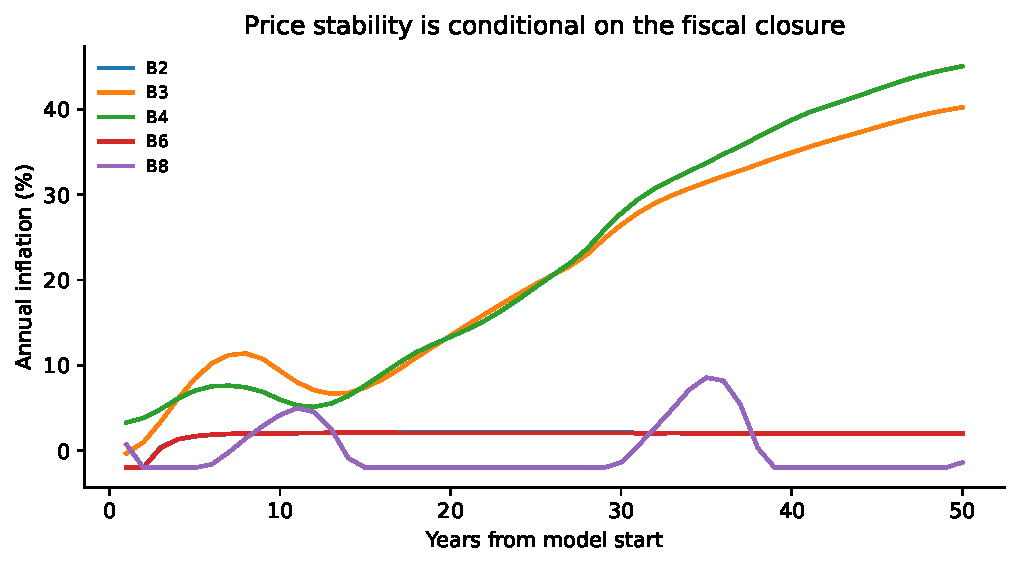
\includegraphics[width=.92\linewidth]{figures/inflation_paths.pdf}
\caption{Inflation under alternative fiscal--monetary closures. A near-target hybrid path is conditional on residual taxation and the stipulated price mechanism.}
\end{figure}
\begin{figure}[htbp]\centering
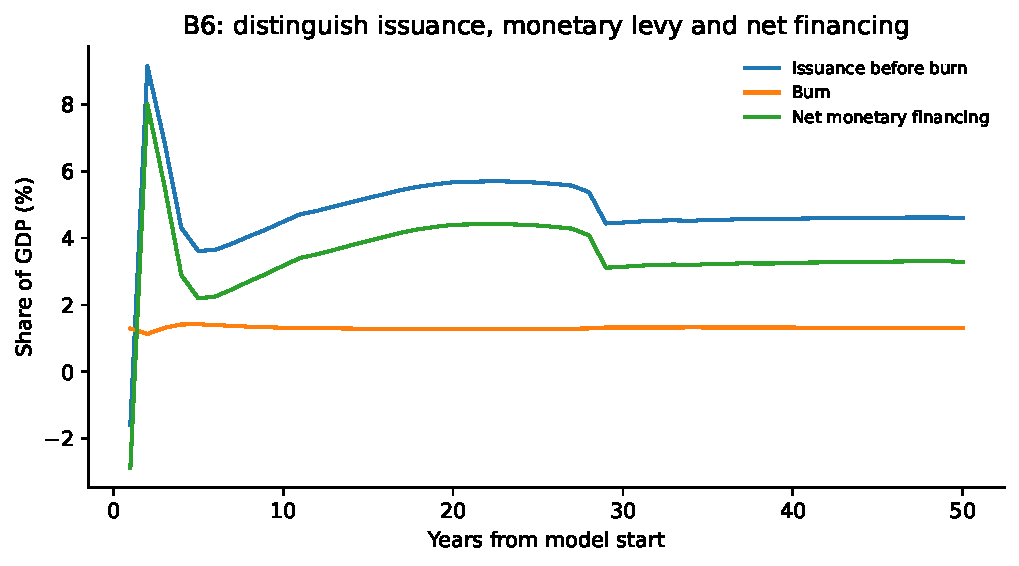
\includegraphics[width=.92\linewidth]{figures/monetary_flows.pdf}
\caption{Hybrid monetary flows. The difference between issuance before burn and net monetary financing is the holding levy. These flows are not additive independent sources of free resources.}
\end{figure}

\subsection{Ownership diffusion and distribution}
User equity reaches \ResultPSixUsownershipShare\% by year 50 in the medium path. The wealth Gini is \ResultPSixGiniWealth, against \ResultPTwoGiniWealth\ in B2 and \ResultPOneGiniWealth\ in the no-transfer comparator. The relevant wealth measure is real transaction balances plus book-valued corporate equity, not an estimate of total EU household wealth. The central synthetic initial distribution is highly concentrated, so the absolute Gini levels should not be read as calibrated observations.

The B5/B6 comparison isolates much of the levy increment. Without special demurrage, B5 reaches a wealth Gini of \ResultPFiveGiniWealth\ and MVI of \ResultPFiveMviGdp\% of GDP. B6's extra levy lowers the conventional tax requirement, but its wealth Gini is slightly higher. Thus this experiment attributes most of the ownership effect to equity diffusion, not to programmable monetary decay. Equal firm-specific grants in B7 achieve a lower Gini and smaller transfer requirement than contribution weighting, at the cost of dropping the proposed link between individual participation and grants. That is an objective trade-off, not a reason to silently redefine usownership.

\begin{figure}[htbp]\centering
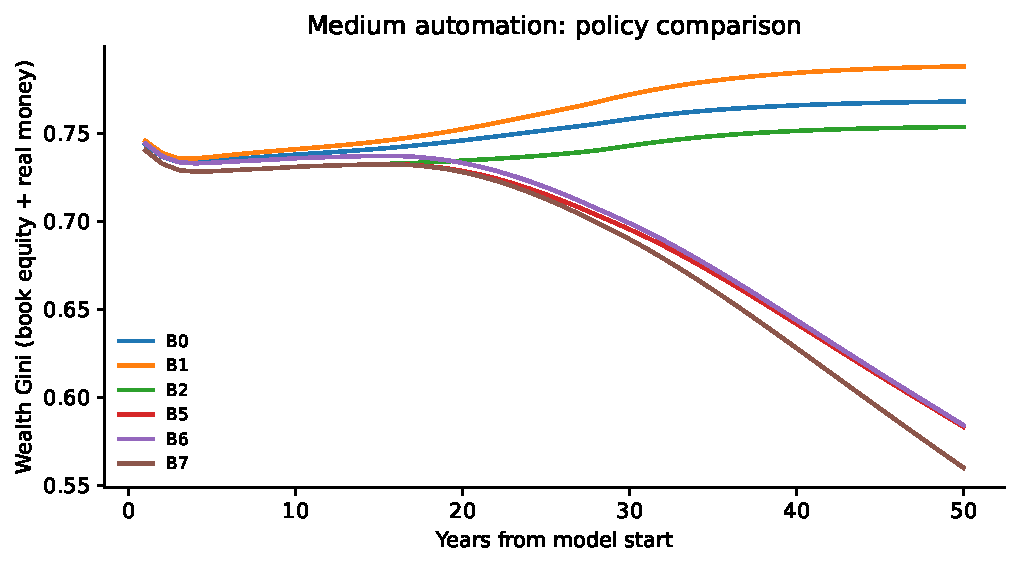
\includegraphics[width=.92\linewidth]{figures/wealth_paths.pdf}
\caption{Wealth distribution in the medium path. Levels depend on the synthetic starting distribution; comparisons hold the accounting and initial draws fixed.}
\end{figure}
\begin{figure}[htbp]\centering
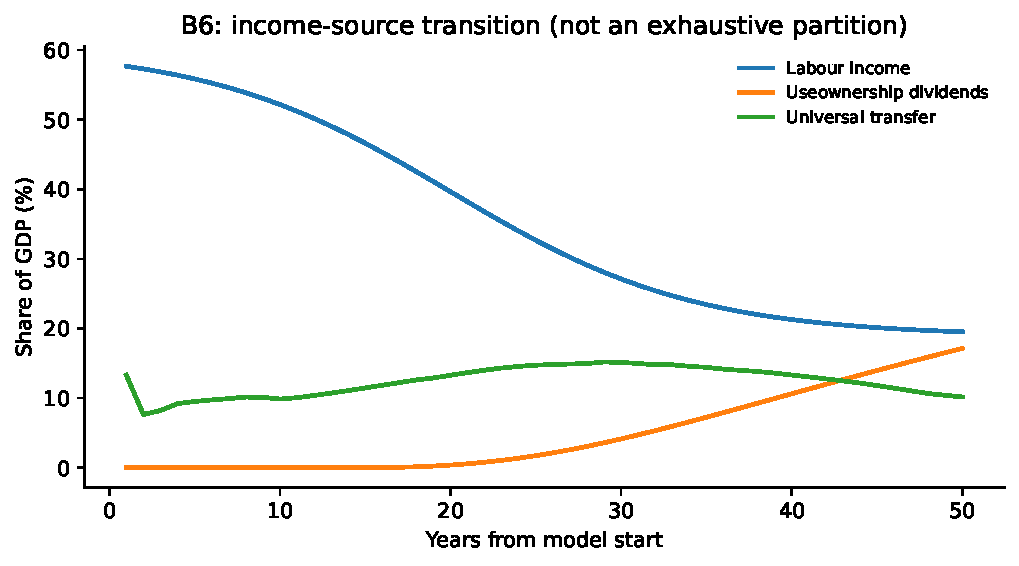
\includegraphics[width=.92\linewidth]{figures/income_transition.pdf}
\caption{The hybrid's income-source transition. Labour, user dividends and transfers are shown separately; ordinary dividends and taxes mean these curves are not an exhaustive GDP partition.}
\end{figure}

\subsection{The transfer peak and the conditional sunset}
The medium B6 path's transfer/GDP ratio peaks at approximately 15.19\% in model year 29, then falls to 10.16\% at year 50. It drops below 1\% around year 82 in the extension and reaches zero by year 100. Slow automation still requires about 8.02\% of GDP at year 100. Fast automation attains greater user ownership and a zero quantile-based transfer by that horizon. These are conditional trajectories under unchanged institutions and synthetic cohorts, not dated forecasts of Europe.

The main pattern does support a gradual ownership bridge, but not an automatic rapid one. A 2\% annual maximum issue is much slower than an immediate ownership redistribution, particularly because the threshold delays issuance. Grant recipients also continue to be heterogeneous. The time at which an aggregate transfer becomes small depends on the floor, payout share, tax incidence and lower-tail participation, not just the aggregate value of automated capital.

\begin{table}[htbp]\centering\small
\caption{Hybrid scenario horizons: no compulsory pooling at any horizon}
\begin{tabular}{lllllll}
\toprule
AI path & Year & Real GDP & User equity & MVI/GDP & Tax/GDP & Wealth Gini \\
\midrule
slow & 10 & 1.18 & 0.0\% & 9.4\% & 27.5\% & 0.737 \\
slow & 25 & 1.56 & 0.0\% & 10.1\% & 27.8\% & 0.740 \\
slow & 50 & 2.72 & 2.8\% & 13.7\% & 31.3\% & 0.731 \\
slow & 100 & 7.25 & 33.2\% & 8.0\% & 26.0\% & 0.559 \\
medium & 10 & 1.31 & 0.0\% & 9.9\% & 26.9\% & 0.736 \\
medium & 25 & 2.69 & 3.9\% & 14.7\% & 30.6\% & 0.719 \\
medium & 50 & 6.48 & 29.7\% & 10.2\% & 27.1\% & 0.584 \\
medium & 100 & 17.67 & 66.3\% & 0.0\% & 18.1\% & 0.371 \\
fast & 10 & 1.72 & 0.8\% & 14.4\% & 32.2\% & 0.733 \\
fast & 25 & 2.72 & 19.0\% & 14.3\% & 31.3\% & 0.648 \\
fast & 50 & 6.41 & 46.6\% & 4.7\% & 21.6\% & 0.490 \\
fast & 100 & 35.79 & 76.7\% & 0.0\% & 17.2\% & 0.311 \\
\bottomrule
\end{tabular}

\par\smallskip\footnotesize Years are elapsed model years. Output multipliers over 100 years are scenario arithmetic, not forecasts. Demography, firm turnover and new generations are not included.
\end{table}

A fixed-real-floor experiment produces an earlier sunset than the prosperity-indexed floor. A lower relative floor of 15\% also reaches a negligible transfer within the fifty-year window, whereas a 40\% relative floor leaves about 30.63\% of GDP in transfers at year 50. These differences are economically substantive. A policy that protects only an initial subsistence basket is not equivalent to a policy allowing displaced households to share proportionately in AI-driven prosperity.

\begin{figure}[htbp]\centering
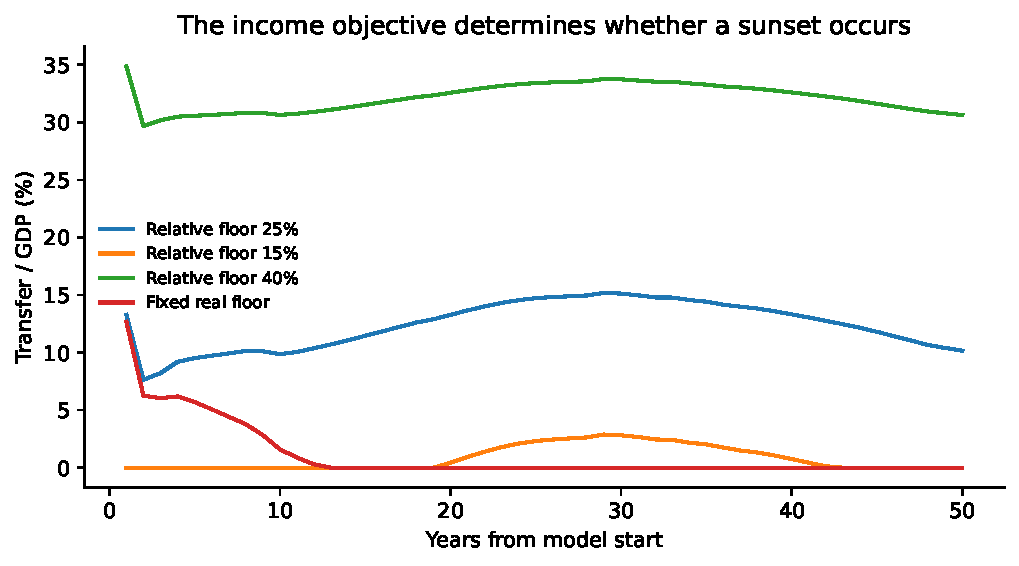
\includegraphics[width=.92\linewidth]{figures/sunset_conditions.pdf}
\caption{Different income objectives give different sunset conclusions. A shrinking transfer ratio is not alone evidence of equitable participation in abundance.}
\end{figure}

\subsection{Coverage, manipulation and reconcentration}
Excluding the lowest-initial-wage 20\% of synthetic participants from equity grants leaves aggregate user equity unchanged but raises year-50 MVI to about 19.15\% of GDP, nearly the B2 no-usownership requirement. This illustrates the coverage condition in the main paper: total ownership diffusion and adequate coverage are distinct. The low contributors still receive the separate universal transfer; the experiment does not endorse conditioning their basic support on participation.

Consumption-only allocation produces a year-50 wealth Gini near 0.660 rather than 0.584. Giving a synthetic attacker 20\% of score mass raises it to about 0.624. Such score capture is not a forecast of a specific bot exploit; it is a stress on measurement integrity. More sophisticated contribution scoring is therefore not automatically more equitable or harder to manipulate than a simple rule.

With immediate permitted liquidation, simulated user equity falls to about 7.72\% and the wealth Gini rises to about 0.753. Ten-year vesting with a 20\% retained core moderates this effect: user equity is about 19.11\% and the Gini about 0.663. These findings are conditional on cash-constrained wealthy buyers and book-value pricing. They identify a reconcentration channel but do not estimate the value of actual legal restrictions or the optimal vesting period.

\begin{figure}[htbp]\centering
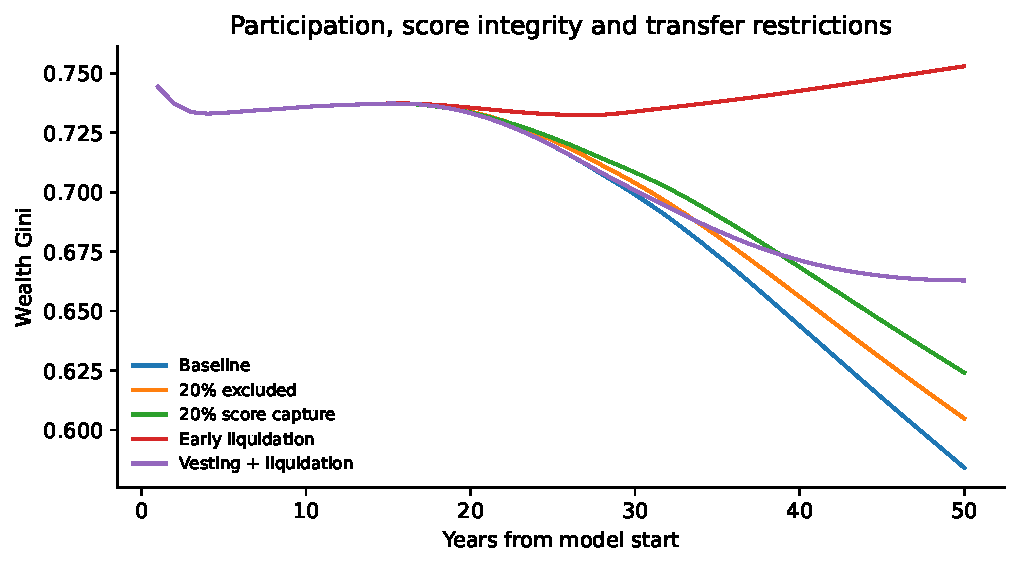
\includegraphics[width=.92\linewidth]{figures/participation_risks.pdf}
\caption{Distributional risks from exclusion, score capture and secondary liquidation. The baseline's retained user shares are a substantive institutional assumption.}
\end{figure}

\subsection{Resource and investment trade-offs}
The central resource constraint binds sufficiently strongly that several policies share the same year-50 real-output level. That equality is not a finding that ownership has no productivity cost; it is partly a property of the binding ceiling. Removing that binding ceiling exposes the assumed investment penalty. At year 50, real GDP is approximately 6.862 with zero dilution penalty, 6.738 with the central penalty and 6.227 with the high penalty. Increasing the penalty can raise current distributable profits by reducing retained investment and can therefore reduce MVI even while long-run output deteriorates. Judging success solely by a smaller transfer bill would reward that undesirable outcome.

The resource envelope also explains why the fast-automation path need not dominate medium automation at every finite date. Greater automation can tighten the assumed resource intensity constraint before later capital/productivity growth changes which constraint binds. No ranking of real-world AI development speeds follows from that particular functional form. The point is to make non-monotonicity and bottlenecks visible rather than to guarantee abundance by construction.

\begin{figure}[htbp]\centering
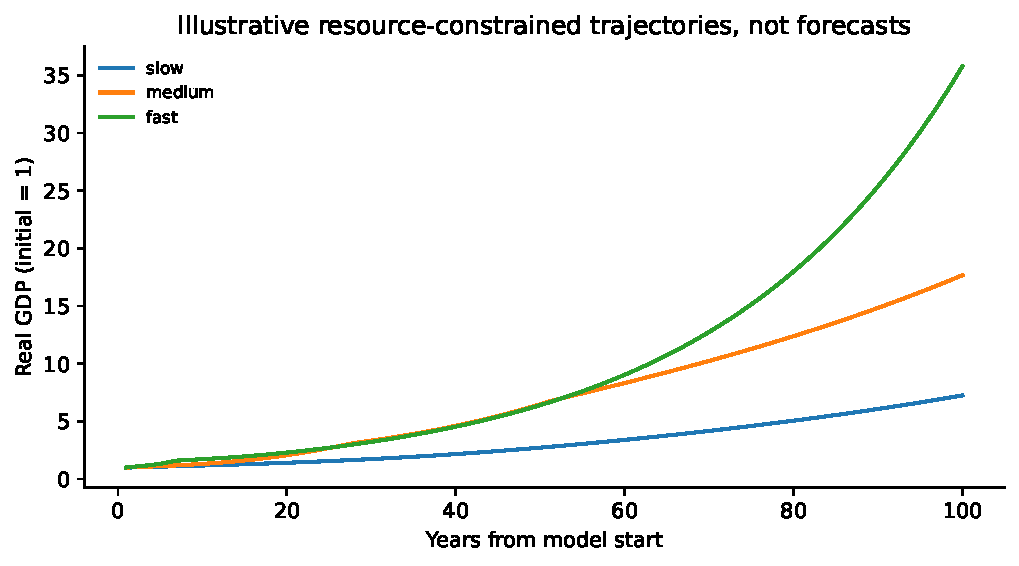
\includegraphics[width=.92\linewidth]{figures/real_output.pdf}
\caption{Resource-constrained scenario trajectories. A century-scale multiplier depends on compounded assumptions and should not be described as a forecast.}
\end{figure}

